\chapter{绪论}
\label{cha:intro}

\section{课题研究背景}
根据中国互联网络信息中心(CNNIC)统计,截至2017年12月,网络直播用户规模达到4.22亿;其中,游戏直播用户规模达到2.24亿,较2016年底增加7756万,占网民总体的29\%,真人秀直播用户规模达到2.2亿,较去年底增加7522万
,占网民总体的28.5\%~\cite{CNNIC}。而据思科公司的数据预测,2016年到2021年的5年间网络直播会增长15倍,到2021年底网络直播会占总视频流量的13\%~\cite{Cisco2017}。目前工业界出现了许多大型的直播平台,比如,国内有斗鱼~\cite{Douyu},熊猫tv~\cite{Panda},国外以Twitch为首的游戏直播平台,具有社交性质的Facebook Live~\cite{Facebook}、Periscope~\cite{Periscope}等,如图~\ref{fig:platform}所示。 而移动网民数量的快速增长,推动直播行业的发展转移到移动端,从2016年下半年开始,移动直播用户赶超PC端用户。大量的统计数据表明,网络直播会成为互联网中越来越重要的存在,而移动直播作为其中占比较大的部分,研究如何优化移动直播的用户体验质量有着重要意义。

\begin{figure}[t]% use float package if you want it here
  \centering
  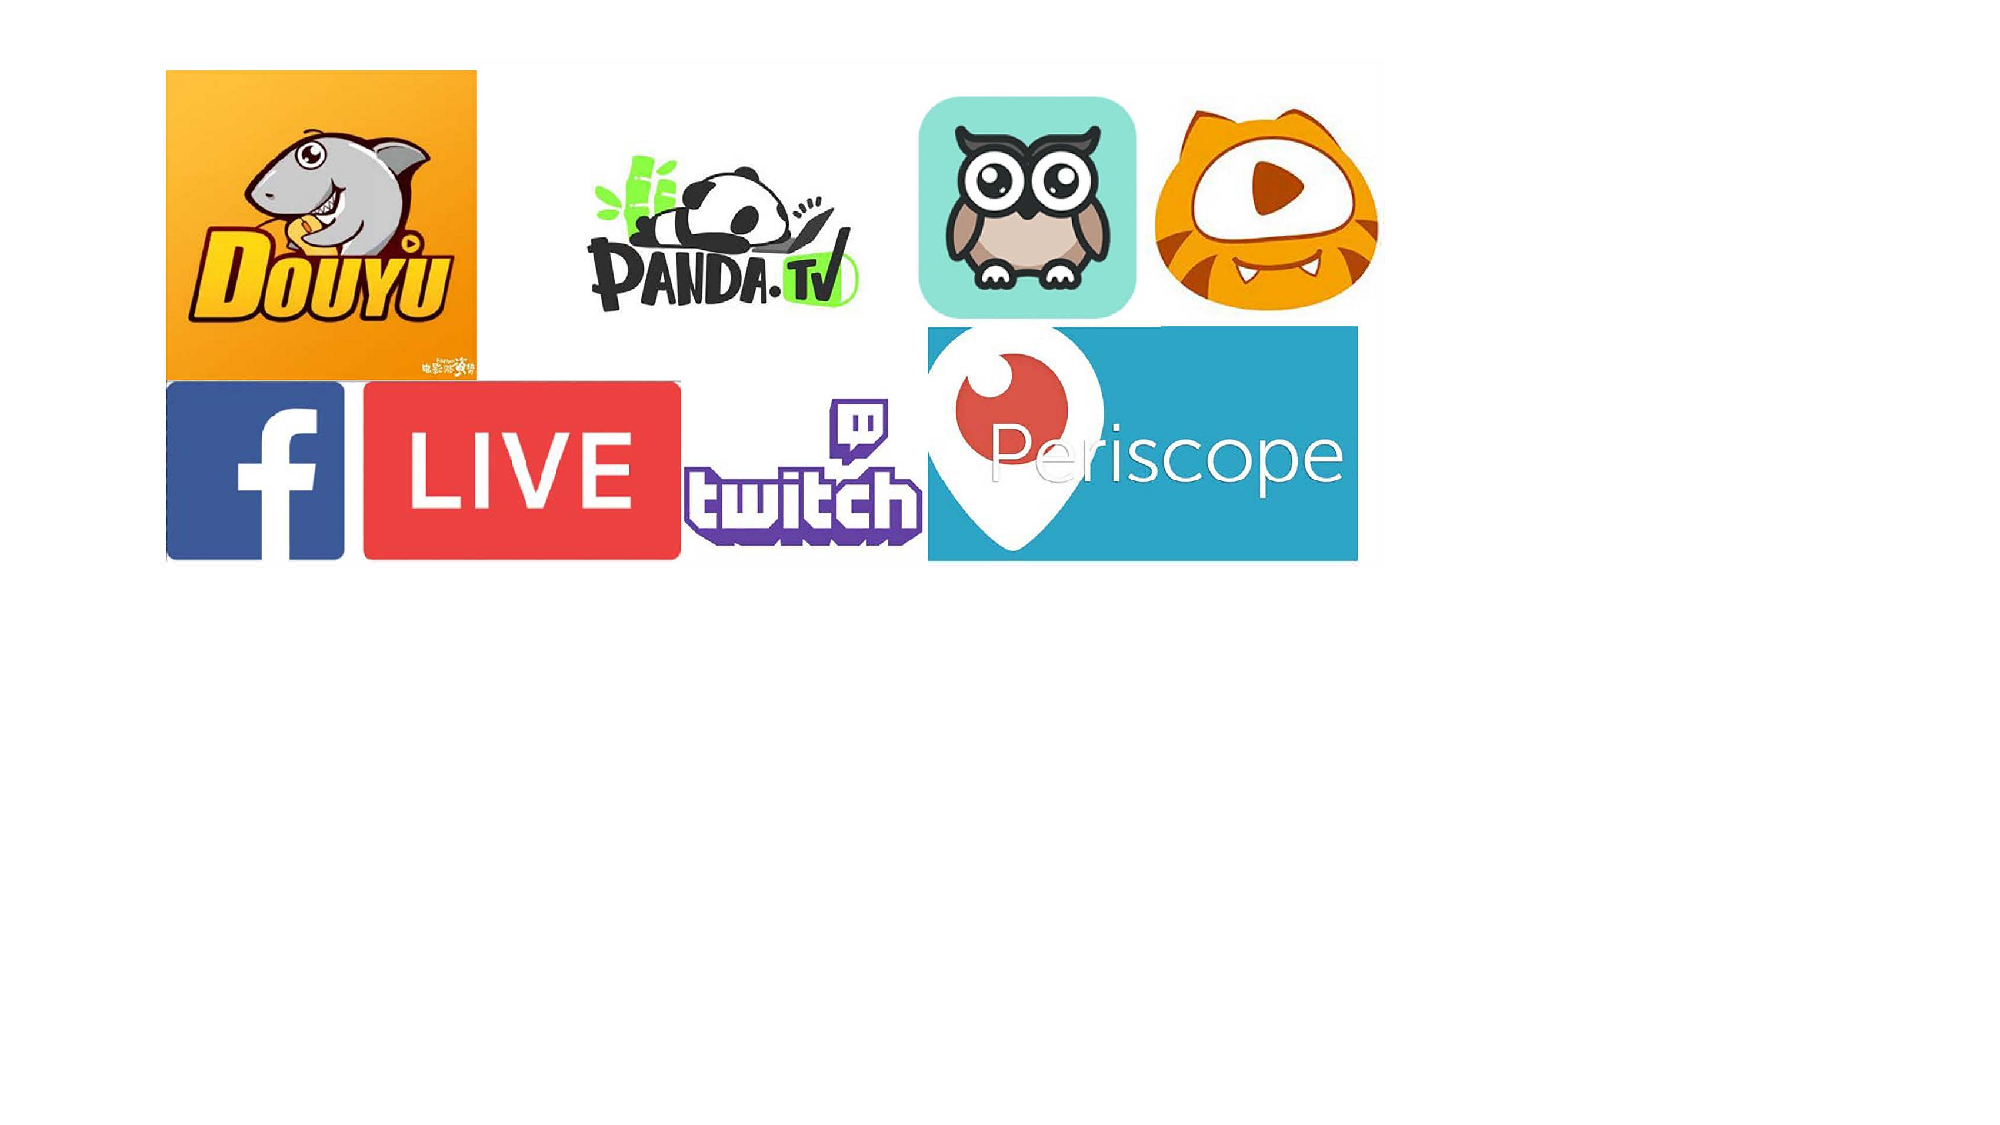
\includegraphics[width=0.7\textwidth]{platform}
  \caption{流行的直播商业平台}
  \label{fig:platform}
\end{figure}

现在火爆的交互直播是由最开始的传统直播演变而来。传统的直播一般只针对“重大事件”,比如ESPN的篮球比赛,奥运会直播等等。传统直播一般预先知道直播的具体时间,运营商会提前为直播源分配好优质充足的链路资源,供直播源上传视频至直播源服务器;源服务器接收到直播视频流后,可能会对接收到的视频流进行一定的转码操作,将RTMP流转码为HTTP流,也可能会将原先单一码率的视频分别编码为多种码率,储存在源服务器上;之后源服务器将编码完的视频,选择合适的码率通过CDN网络,IP组播和P2P~\cite{zhang2005coolstreaming}等分发技术分发到每个CDN边缘节点;观看直播的用户从CDN边缘节点处获取视频。传统直播一般全程使用HTTP协议,为了应对可能出现的网络状况变化,保证用户观看的连续性,传统直播一般会把发送和接收缓存都设置得比较大,导致端到端的时延也较大,为几十秒左右。但随着移动设备的普及,用户已经不再满足于单纯的观看直播,用户开始逐渐成为直播内容的贡献者,传统直播技术此时不再能够满足用户的需求。同时由于LTE等通信技术的发展,低延迟的个人交互直播应运而生,繁荣发展。

RTMP(Real Time Message Protocol),即实时消息传送协议,用于传递音频信息以及视频信息。RTMP协议因其较低的端到端时延在交互直播中得到了广泛应用。RTMP是一种面向连接的实时流式传输协议,在传输开始前RTMP层首先要握手先建立连接,面向连接的传输协议保证了传输的安全性。消息是RTMP传输协议的基本数据单元,消息包含音频信息和视频信息,一般将一个视频帧封装成一个视频消息。而HTTP协议的基本传输数据单元是一个视频块,视频块时长一般为4-10s,只有当完整接收到一个视频块之后,用户端才能正常播放。以视频帧作为RTMP协议的基本传输单元,RTMP协议对应的端到端延时较小。RTMP协议低延时的特性使得它被应用在许多商业直播平台上面,包括Facebook Live, Periscope,熊猫TV,斗鱼等国内外大型直播平台。

尽管学术界目前有很多研究都关注于提升直播用户的体验质量,但很少有人研究在直播应用中,通过优化主播端的上传质量,从而去优化用户的观看质量。但对于直播应用来说,主播端的视频传输质量非常重要。如图~\ref{fig:architecture}所示,主播端在直播架构中占据着源头的地位,所以主播端的任何延迟或者上传失败都会随着分发网络传递到用户端,影响着全部用户的观看体验质量。除此之外,主播端为用户观看到的视频传输质量设了一个上限,下游用户的质量不可能超过主播端的质量。因此,主播端需要在可能的情况下上传尽量高清的视频。

\section{主要研究目标和贡献}
个人直播应用虽然由传统直播演变而来,但也不同于传统的直播应用。传统的直播应用的源服务器处上传带宽相对充足稳定,端到端的传输时延一般会在几十秒的量级。但在个人交互直播中,大多数的主播端可能会使用无线网络进行直播,同时由于移动直播中主播端不固定的特性,网络抖动会比较剧烈,网络带宽不稳定。另外,交互直播要求端到端的时延必须在几秒以下,才能满足主播和观众互动的要求。比如,有观众给主播提问或者送礼物,主播需要及时的回应,否则可能会打击观众的积极性。交互直播的这些特性为主播端传输优化带来了新的挑战,可以总结为一句话:在抖动的带宽环境下尽量提供较高的传输质量和用户体验,包括视频质量和端到端的延时等要求。

对于个人交互直播来说,无线网络环境可能会带来新的质量问题。为了验证是否现有的直播平台能否有效的应对无线网络环境,我们首先进行了一定的测量实验。我们选择了两个流行的直播应用,斗鱼和Twitch,通过在主播端控制带宽变化,监控主播的出口吞吐量,发现这些直播平台都普遍存在着两个质量问题:
\begin{enumerate}
  \item 短暂的网络带宽抖动在应用层会产生放大效应,从而导致长时间的视频质量下降。测量过程中,我们发现如果主播端发生了1s的网络抖动,那么应用层观测到的结果是主播端会有数秒的上传暂停的情况出现。因为交互直播要求端到端的时延尽量小,所以系统各个部分的缓存都很小,暂停数秒上传反映到观众端,则是几秒的黑屏或者暂停。
  \item 现有的直播平台都无法有效应对带宽长时间降低的状况。由于设备移动的原因,可能导致小区间切换,WiFi和蜂窝网切换等问题,主播端经常会出现长时间的带宽波动。但经过我们的测量发现,目前的商业实现都不能有效的解决这个问题。目前的商业平台在带宽降低的状况下,依然维持着初始的码率,视频产生速率远远高于网络容量,从而引起严重的视频质量下降。
\end{enumerate}

通过对开源直播应用源码的分析发现,应用层的放大效应是由于RTMP协议的丢包行为导致。当视频帧的队列溢出时,主播端会主动丢包,丢包导致剩下的一些视频帧无法解码,从而用户端会观测到长时间的视频卡顿。而且,一些简单直接的方案,例如,增大视频帧队列的长度,或者换用其他的丢包方式,都会带来一定的质量损失,或者增大端到端的时延,或者降低视频的质量。比如,增大主播端的视频队列长度,可以很好的解决短暂的带宽下降,但端到端的最高时延也会相应的增大。

另外,对于长时间的网络带宽降低,一个可能的解决方案是码率自适应带宽。但现有的方法都集中在研究点播场景下的自适应码率,这些在点播领域效果比较好的自适应码率方案,在主播端表现不好,因为点播情况下视频的队列长度一般维持在10s左右。而主播端的视频队列通常只有1s左右。由于更小的视频队列长度,主播端准确的码率自适应更加具有挑战性。

本文中,我们提出了一整套的解决方案,简称为GVBR(Greedy Variable Bitrate Solution),大大提高了交互直播中主播端的视频质量。我们的主要出发点是主播端的质量问题可以通过跨层协同设计来解决。GVBR主要包括三层,RTMP层,GoP级别,以及帧级别,三个级别的优化目标都是保证视频的质量和及时性。 RTMP层的配置调整主要是去选择最优的关键帧间隔,因为过小的关键帧间隔会导致视频压缩比过高,视频质量损失,而过大的关键帧间隔会导致放大效应带来的丢帧过多;GOP层面根据预测的带宽和视频帧队列数据量去自适应选择每个GOP的码率;帧级别的解决方案主要是一个智能丢帧策略,尽可能多的减少放大效应。虽然我们的整套解决方案修改了视频流协议的两层,但所有的改动都不用修改内部逻辑,或者是更改可调的参数(例如,关键帧间隔),或者是改变软件中的控制逻辑(丢帧的逻辑和码率自适应策略)。

通过仿真,我们说明好的RTMP层协议可以大大的提高视频质量。通过改变关键帧间隔,我们测量不同关键帧间隔对应的视频质量和丢帧数,给出关键帧的最优选择范围;智能丢帧策略与离线最优算法和默认丢帧策略做对比,相比于默认策略减少了15\%的丢帧,和最优策略有5\%的差距。本文选择了动态码率在点播领域最新的两个算法作为对比算法,与我们提出的算法GVBR作对比。通过在不同网络环境下的大规模仿真,我们发现GVBR同目前现先进的算法比,可以减少至少50\%的丢帧;而相比原始默认的算法,在保证同样视频码率的情况下,视频卡顿的概率减少90\%。

总而言之,本文有两个主要的贡献点:
\begin{itemize}
  \item 我们是第一个把目光着眼于提升主播端视频质量的。通过对于流行视频直播平台的测量,我们发现主播端普遍存在两个质量问题,网络层短暂的带宽波动会在应用层导致长时间的视频卡顿,并且现在的直播应用都无法有效解决长时间的带宽波动。
  \item 我们提出了一整套解决方案,去协同解决观测到的视频质量问题,包括帧编码参数和智能丢帧策略,以及GOP级别的比特率自适应策略。
\end{itemize}

\section{文章组织架构}
本文的内容共有六章,按照如下方式展开:

第一章是绪论部分,主要介绍交互直播的发展过程,简要概率了我们的研究目标。

第二章介绍了直播相关的一些背景知识,主要包括个人直播的架构、特点、以及性能要求。

第三章从我们搭建的平台出发,给出测量中发现的问题,目前的直播平台并不能很好的满足性能要求;并给出在商业平台中的测量,实验发现商业平台也不能很好的解决上述问题。

第四章,剖析直播软件的源码,发现上述问题出现的原因,主要是由于视频编码输出的码率不能实时的按照带宽变化,最后我们给出了一些优化设计的原则。

第五章根据设计准则,我们设计了一整套的解决方案,涵盖帧级到GoP级。

第六章与之前的算法进行比较,进行充分的实验仿真。

第七章总结现有的工作,并展望未来的研究方向。

